\RequirePackage[orthodox]{nag}
\documentclass[11pt]{article}

%% Define the include path
\makeatletter
\providecommand*{\input@path}{}
\g@addto@macro\input@path{{include/}{../include/}}
\makeatother

\usepackage{../../include/akazachk}


\title{ECH4905 ChemE Optimization HW 6}
\author{Andres Espinosa}

\begin{document}
\maketitle

\section{Problem 1}
Consider the following problem:

\[
\text{minimize } 
\begin{aligned}
    Z_1(\mathbf{x}) &= x_1^2 + x_2^2 + x_3^2 + x_4^2 + x_5^2, \\
    Z_2(\mathbf{x}) &= 3x_1 + 2x_2 - x_3^3 + 0.01(x_4 - x_5)^3,
\end{aligned}
\]

\[
\text{subject to:}
\]
\[
\begin{aligned}
    x_1 + 2x_2 - x_3 - 0.5x_4 + x_5 &= 2, \\
    4x_1 - 2x_2 + 0.8x_3 + 0.6x_4 + 0.5x_5^2 &= 0, \\
    x_1^2 + x_2^2 + x_3^2 + x_4^2 + x_5^2 &\leq 10.
\end{aligned}
\]

\subsection{Part A}
Use the epsilon-constraint method to solve the above nonlinear programming (NLP) problem in GAMS. Upload your code.

\textbf{Solution:}
To solve this with the epsilon-constraint method, we can take the first objective $Z_1$ and set that as our primary objective, while we take the second objective $Z_2$ and turn that into a constraint.
The optimization problem now looks like this:

\begin{align*}
  \text{minimize} & \quad Z_1(\textbf{x}) = x_1^2 + x_2^2 + x_3^2 + x_4^2 + x_5^2 \\
  \text{subject to} & \quad x_1 + 2x_2 - x_3 - 0.5x_4 + x_5 = 2, \\
  & \quad 4x_1 - 2x_2 + 0.8x_3 + 0.6x_4 + 0.5x_5^2 = 0, \\
  & \quad x_1^2 + x_2^2 + x_3^2 + x_4^2 + x_5^2 \leq 10 \\
  & \quad 3x_1 + 2x_2 - x_3^3 + 0.01(x_4 - x_5)^3 \leq \varepsilon
\end{align*}
Below is the GAMS code that was used for this problem.
\begin{verbatim}
Sets
n / 1*30 /;

Parameters
epsilon_n(n)
pareto_z1(n)
pareto_z2(n);

Scalars
    z2_min
    z2_max
    epsilon /1/;


Variables
x_1
x_2
x_3
x_4
x_5
z_1
z_2;

x_1.lo = -4;   x_1.up = 4;
x_2.lo = -4;   x_2.up = 4;
x_3.lo = 0;   x_3.up = 4;
x_4.lo = -4;   x_4.up = 4;
x_5.lo = -4;   x_5.up = 4;

z_1.lo = -1000; z_1.up = 1000;
z_2.lo = -1000; z_2.up = 1000;


Equations
z_1_eq
z_2_eq
constraint_1
constraint_2
constraint_3
non_neg_power_constraint
epsilon_constraint
;
z_1_eq.. z_1 =e= x_1**2 + x_2**2 + x_3**3 + x_4**2 + x_5**2;
z_2_eq.. z_2 =e= 3*x_1 + 2*x_2 - x_3**3 + 0.01*(x_4 - x_5)**3;
constraint_1.. x_1 + 2*x_2 - x_3 - 0.5*x_4 + x_5 =e= 2;
constraint_2.. 4*x_1 - 2*x_2 + 0.8*x_3 + 0.6*x_4 + 0.5*x_2**2 =e= 0;
constraint_3.. z_1 =l= 10;
non_neg_power_constraint.. x_4 =g= x_5;
epsilon_constraint.. z_2 =l= epsilon;

Model FullModel / all / ;
model BoundedModel / all - epsilon_constraint / ;

option NLP=baron;
option optcr = 0.00001;
option limrow = 4000;

* First, solve BoundedModel to get min and max z_2
solve BoundedModel using MINLP minimizing z_1;
z2_min = z_2.l;

solve BoundedModel using MINLP minimizing z_2;
z2_max = z_2.l;

* Now loop to build Pareto front
loop(n,
    epsilon_n(n) = z2_min + (z2_max - z2_min)*(ord(n)-1)/(card(n)-1);
    epsilon = epsilon_n(n);
    solve FullModel using MINLP minimizing z_1;
    pareto_z1(n) = z_1.l;
    pareto_z2(n) = z_2.l;
);

* Save results
execute_unload 'pareto_front.gdx', pareto_z1, pareto_z2, epsilon_n;
\end{verbatim}
\subsection{Part B}
Create a plot with the Pareto front.

\textbf{Solution:} 
The plot is available in Figure~\ref{fig:prob1_pareto}

\begin{figure}[htbp]
  \centerline{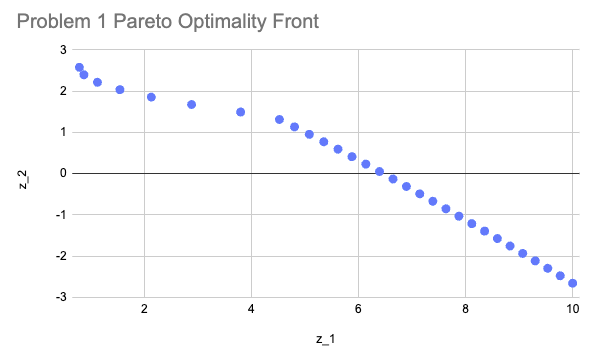
\includegraphics[width=0.75\textwidth]{images/prob1_pareto.png}}
  \caption{Problem 1 Pareto Chart}
  \label{fig:prob1_pareto}
\end{figure}

\section{Problem 2}
Consider the same problem that we explored in the previous homework in Figure~\ref{fig:prob2_superstructure}.

\begin{figure}[htbp]
  \centerline{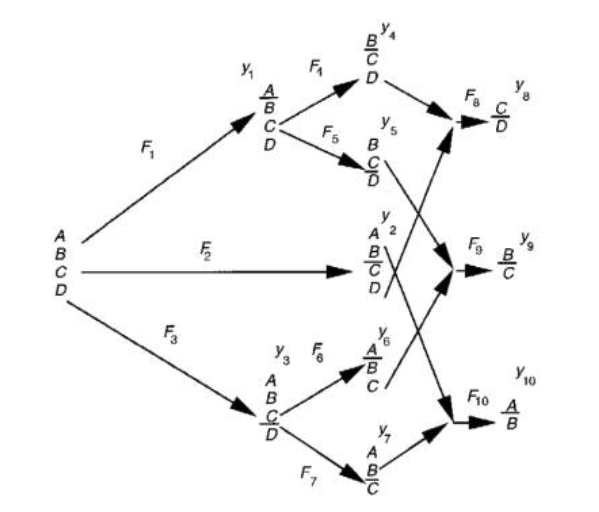
\includegraphics[width=0.50\textwidth]{images/prob2_superstructure.png}}
  \caption{Problem 2 superstructure}
  \label{fig:prob2_superstructure}
\end{figure}

In which the total cost of a distillation column was calculated as follows:

\[
\text{cost}_k = \alpha_k + \beta_k F_k + \gamma_{\text{Hot}} Q_k^{\text{Hot}} + \gamma_{\text{Cold}} Q_k^{\text{Cold}},
\]

where:
\begin{itemize}
    \item $\alpha_k$ represents a fixed capital cost,
    \item $\beta_k$ represents the variable investment cost,
    \item $\gamma_{\text{Hot}}$/$\gamma_{\text{Cold}}$ is the cost of hot/cold utilities,
    \item $Q_k^{\text{Hot}}$/$Q_k^{\text{Cold}}$ is the total demand of hot and cold utilities (assume they are equal).
\end{itemize}

Considering an initial feed of $1000$ Kmol/h, and a composition of the feed stream (mole fraction) of $A=0.15$, $B=0.3$, $C=0.35$, and $D=0.2$, and the following data in Figure~\ref{fig:prob2_table}:

\begin{figure}[htbp]
  \centerline{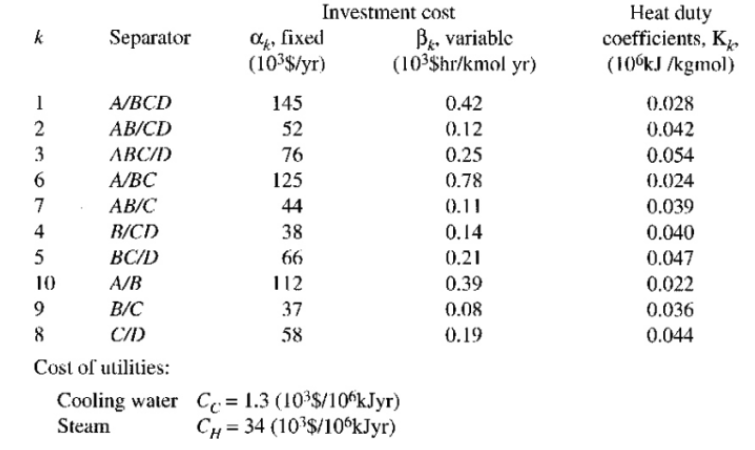
\includegraphics[width=0.75\textwidth]{images/prob2_table.png}}
  \caption{Problem 2 Data table}
  \label{fig:prob2_table}
\end{figure}

\[
\begin{array}{|c|c|c|c|c|}
\hline
\text{Scenario} & \text{Probability} & \gamma_{\text{Hot}} \, (10^3 \, \$/10^6 \, \text{KJ-y}) & \gamma_{\text{Cold}} \, (10^3 \, \$/10^6 \, \text{KJ-y}) \\
\hline
1 & 0.025 & 0.1 & 3 \\
2 & 0.05 & 0.1 & 10 \\
3 & 0.1 & 0.1 & 34 \\
4 & 0.15 & 1.3 & 3 \\
5 & 0.35 & 1.3 & 10 \\
6 & 0.15 & 1.3 & 34 \\
7 & 0.1 & 3 & 3 \\
8 & 0.05 & 3 & 10 \\
9 & 0.025 & 3 & 34 \\
\hline
\end{array}
\]

Unlike the previous case, assume that the parameters $\gamma_{\text{Hot}}$ and $\gamma_{\text{Cold}}$ are known with uncertainty. The probability of occurrence in different scenarios is as follows:




Formulate a stochastic optimization problem in GAMS and solve the problem.

\textbf{Solution:}



\end{document}